%%%%%%%%%%%%%%%%%%%%%%%%%%%%%%%%%%%%%%%%%%%%%%%%%%%%%%%%%%%%%%%%%%%%%%%
% Based on IEEE the conference template available                     %
% at https://www.ieee.org/conferences/publishing/templates.html       %
% Adapted for the Data Science Lab course at Politecnico di Torino    %
% by Giuseppe Attanasio, Flavio Giobergia                             %
% 2020, DataBase and Data Mining Group                                %
%%%%%%%%%%%%%%%%%%%%%%%%%%%%%%%%%%%%%%%%%%%%%%%%%%%%%%%%%%%%%%%%%%%%%%%

\documentclass[conference]{IEEEtran}
\usepackage{cite}
\usepackage{amsmath,amssymb,amsfonts}
\usepackage{algorithmic}
\usepackage{graphicx}
\usepackage{textcomp}
\usepackage{xcolor}

\begin{document}

\title{Particle position prediction \\ using a regression pipeline}

\author{\IEEEauthorblockN{Andrea Cucchietti}
s327134 \\
\IEEEauthorblockA{\textit{Collegio di Ingegneria Informatica,}\\
\textit{del Cinema e Meccatronica} \\
\textit{Politecnico di Torino}\\
s327134@studenti.polito.it}
\and
\IEEEauthorblockN{Shakti Singh Rathore}
s328222 \\
\IEEEauthorblockA{\textit{Collegio di Ingegneria Informatica,} \\
\textit{del Cinema e Meccatronica} \\
\textit{Politecnico di Torino}\\
s328222@studenti.polito.it}
}

\maketitle

\begin{abstract}
RSD is a sensor that tracks the position of passing particles. Throughout this report, we propose a data science pipeline that uses as input several features extracted by the RSD signals, removes the noise and the outliers, and predicts the passing position with a regression model. Three regressors are discussed. The results exceed a naive baseline and the performance of the same models on the original data.
\end{abstract}

\section{Problem overview}
\label{sec:problemOverview}
The group project consists in predicting the position of a particle when it passes through an RSD sensor. The sensor is flat, hence the position is represented by $(x, y)$ values. 
The task has to be performed through a multi-output regression pipeline, one per coordinate. \\
The Resistive Silicon Detector(RSD) sensor is composed of 12 metallic $pads$. They have an asterisk-shape and they can be clearly distinguished in Figure \ref{fig:rsd}.\\

\begin{figure}[htbp]
\centerline{\includegraphics[scale=0.12]{images/RSD_enumerated.pdf}}
\caption{Pads of the RSD sensor and their corresponding signal number}
\label{fig:rsd}
\end{figure}

Each pad records a measure that is transferred and stored by the system. Due to hardware constraints, not all the signals provided are meaningful, but 6 of the 18 readings are noise. \\

We define as $event$ when a particle passes through the sensor. The dataset is composed of 514,000 events divided into:
\begin{itemize}
    \item 385,500 in the $development$ set
    \item 128,500 in the $evaluation$ set
\end{itemize}

All the fields have a not null valid value. Each record contains some features of an event extracted from every signal provided by the RSD sensor. They are:
\begin{itemize}
    \label{lst:typeFeature}
    \item $pmax$: the value of the positive peak of the signal in $mV$
    \item $negpmax$: the value of the negative peak of the signal in $mV$
    \item $area$: the value of the area under the signal
    \item $tmax$: the time between a reference moment and the positive peak in $ns$
    \item $rms$: the root mean square of the signal
\end{itemize}
The signal is represented as a number inside the square brackets at the end of the column name. Therefore, "pmax[0]" means the feature pmax obtained by the signal 0. We are going to use the same notation throughout the report.\\
The position of each event is enforced during the experiments and it is also provided in the development set. On the other hand, the evaluation set contains only the identifier of the events. \\

The algorithms have to exploit the information provided by the development set to predict the position of the events present in the evaluation set. Then, the results are submitted to an online platform, where they are evaluated according to the average Euclidean distance (\ref{eq:EuclideanDist}).
\begin{equation}
    \label{eq:EuclideanDist}
    d=\frac{1}{n} \sum_i \sqrt{(x_i-\hat{x}_i)^2+(y_i-\hat{y}_i)^2}
\end{equation} 

The development set can be used to make some analysis, especially according to the position.\\
\begin{figure}[htbp]
\centerline{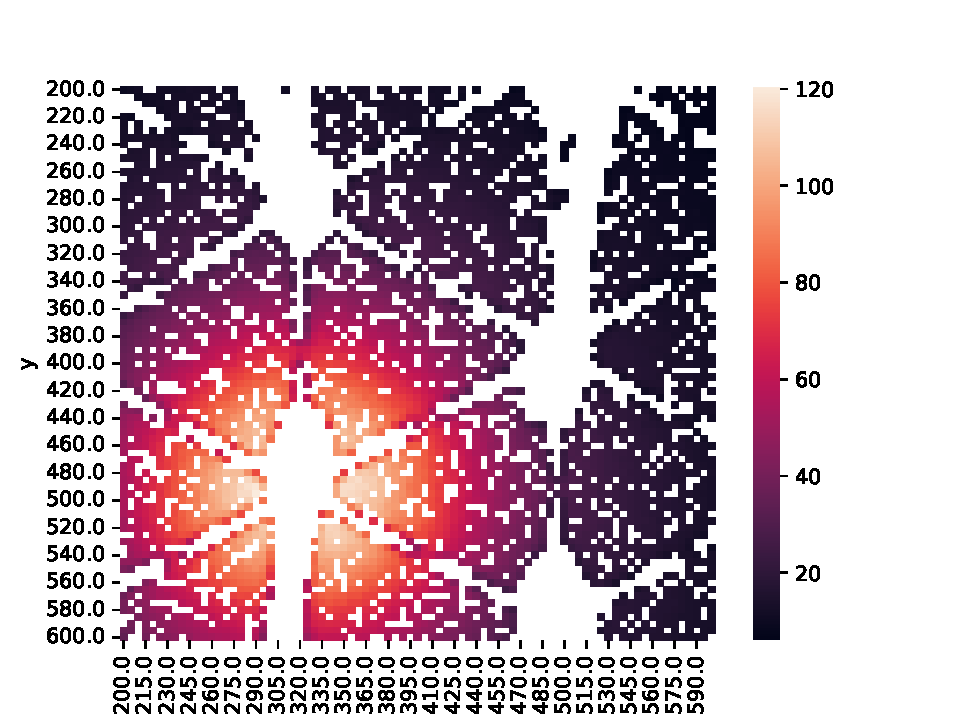
\includegraphics[scale=0.38]{images/pmax[5]_heatmap.pdf}}
\caption{Mean pmax[5] values aggregating by (x, y) the development set}
\label{fig:pmax[5]_heatmap}
\end{figure}
\begin{figure}[htbp]
\centerline{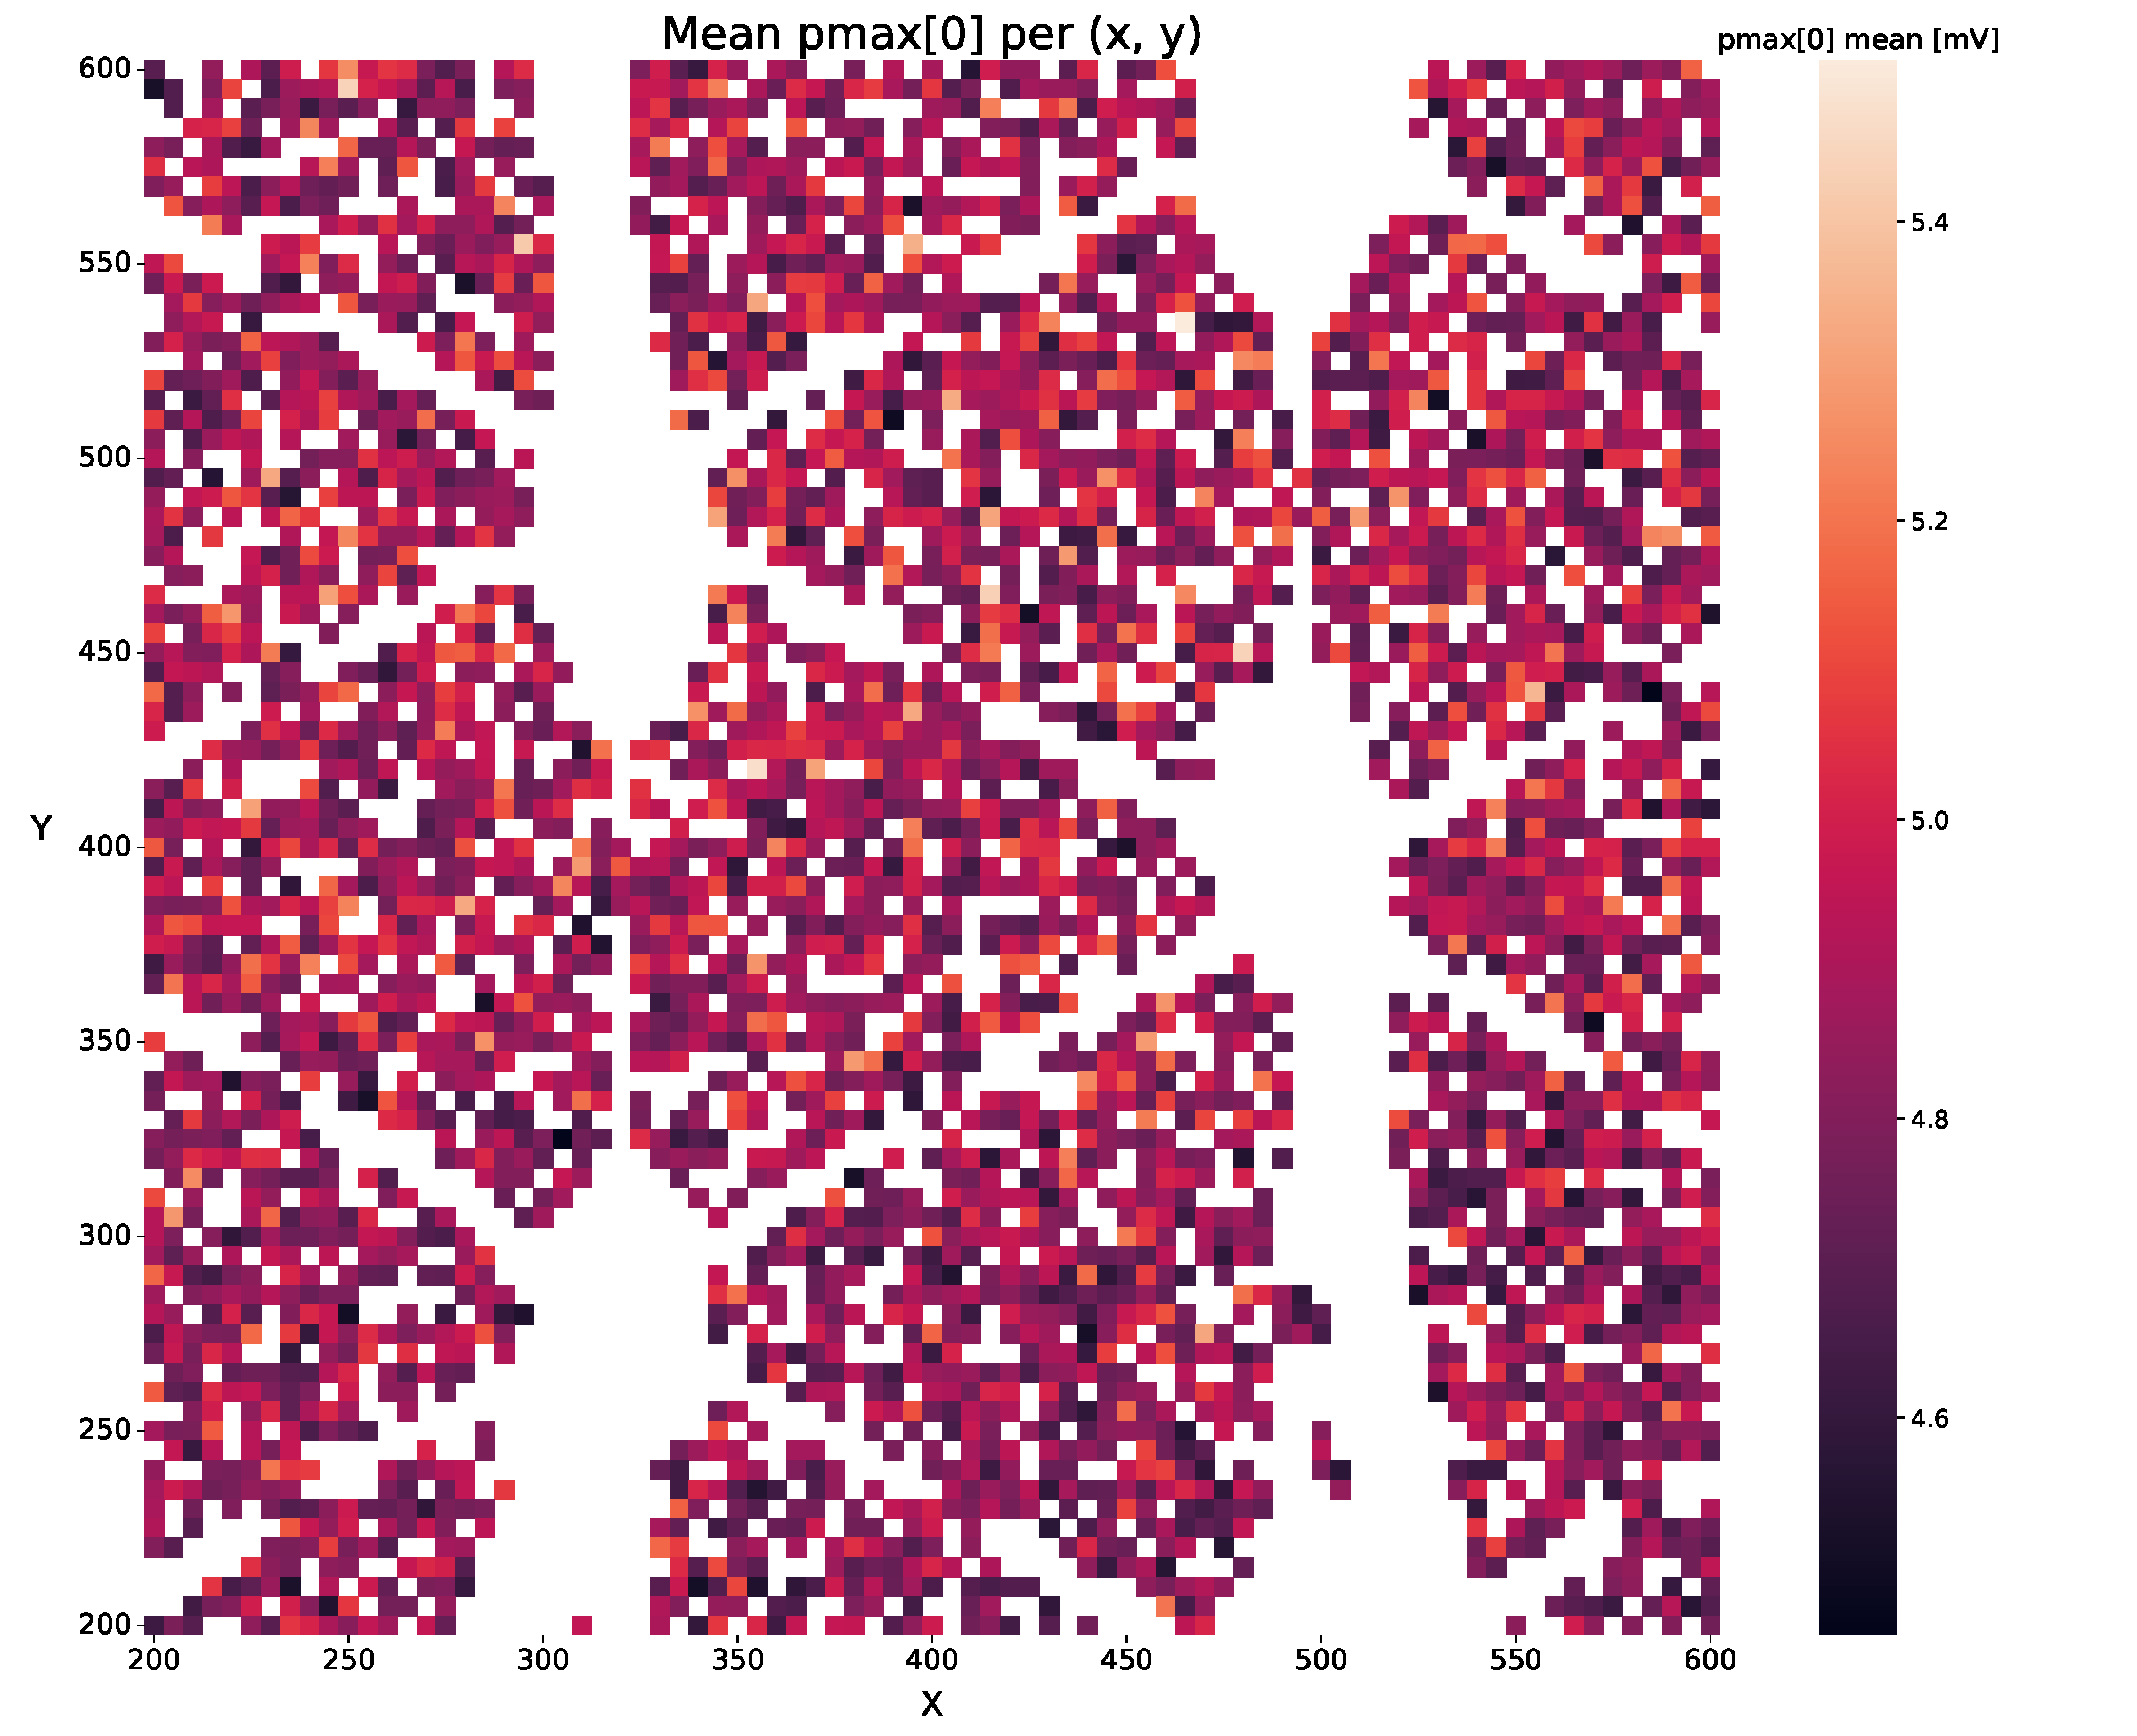
\includegraphics[scale=0.38]{images/pmax[0]_heatmap.pdf}}
\caption{Mean pmax[0] values aggregating by (x, y) the development set}
\label{fig:pmax[0]_heatmap}
\end{figure}
A first observation is that for every $(x, y)$ available in the records, there are 100 events. The x and y values present are all the integers in the range $(200 \mu m, 600 \mu m)$ with step $5 \mu m$. Furthermore, not all the possible $(x, y)$ combinations are present as reported in Figure 
\ref{fig:pmax[5]_heatmap}. In particular, the positions of the pads and the wires can be identified by the complete absence of events. This is a consequence of their reflective properties. Only the shape of a few pads is complete because the positions collected are only in the central zone of the sensor. 

Figure \ref{fig:pmax[5]_heatmap} represents the mean pmax aggregating by $(x, y)$. Comparing the heat maps of the average pmax of different signals was useful for discerning the noise. An example is the difference between Figures \ref{fig:pmax[5]_heatmap} and \ref{fig:pmax[0]_heatmap}. The latter is clearly noise. \\
%(put the Figures of pmax[5] and pmax[0])
The same heat maps were used to identify the pad corresponding to each signal. The mean value of a specific pmax for a given $(x, y)$ is high only if the passing position of the particle is close to the pad. For instance, the pad corresponding to signal 5 is the one surrounded by cells encoded with brighter colors in Figure \ref{fig:pmax[5]_heatmap}.
The pad and the corresponding signal number are represented in Figure \ref{fig:rsd}.\\

\begin{figure}[htbp]
\centerline{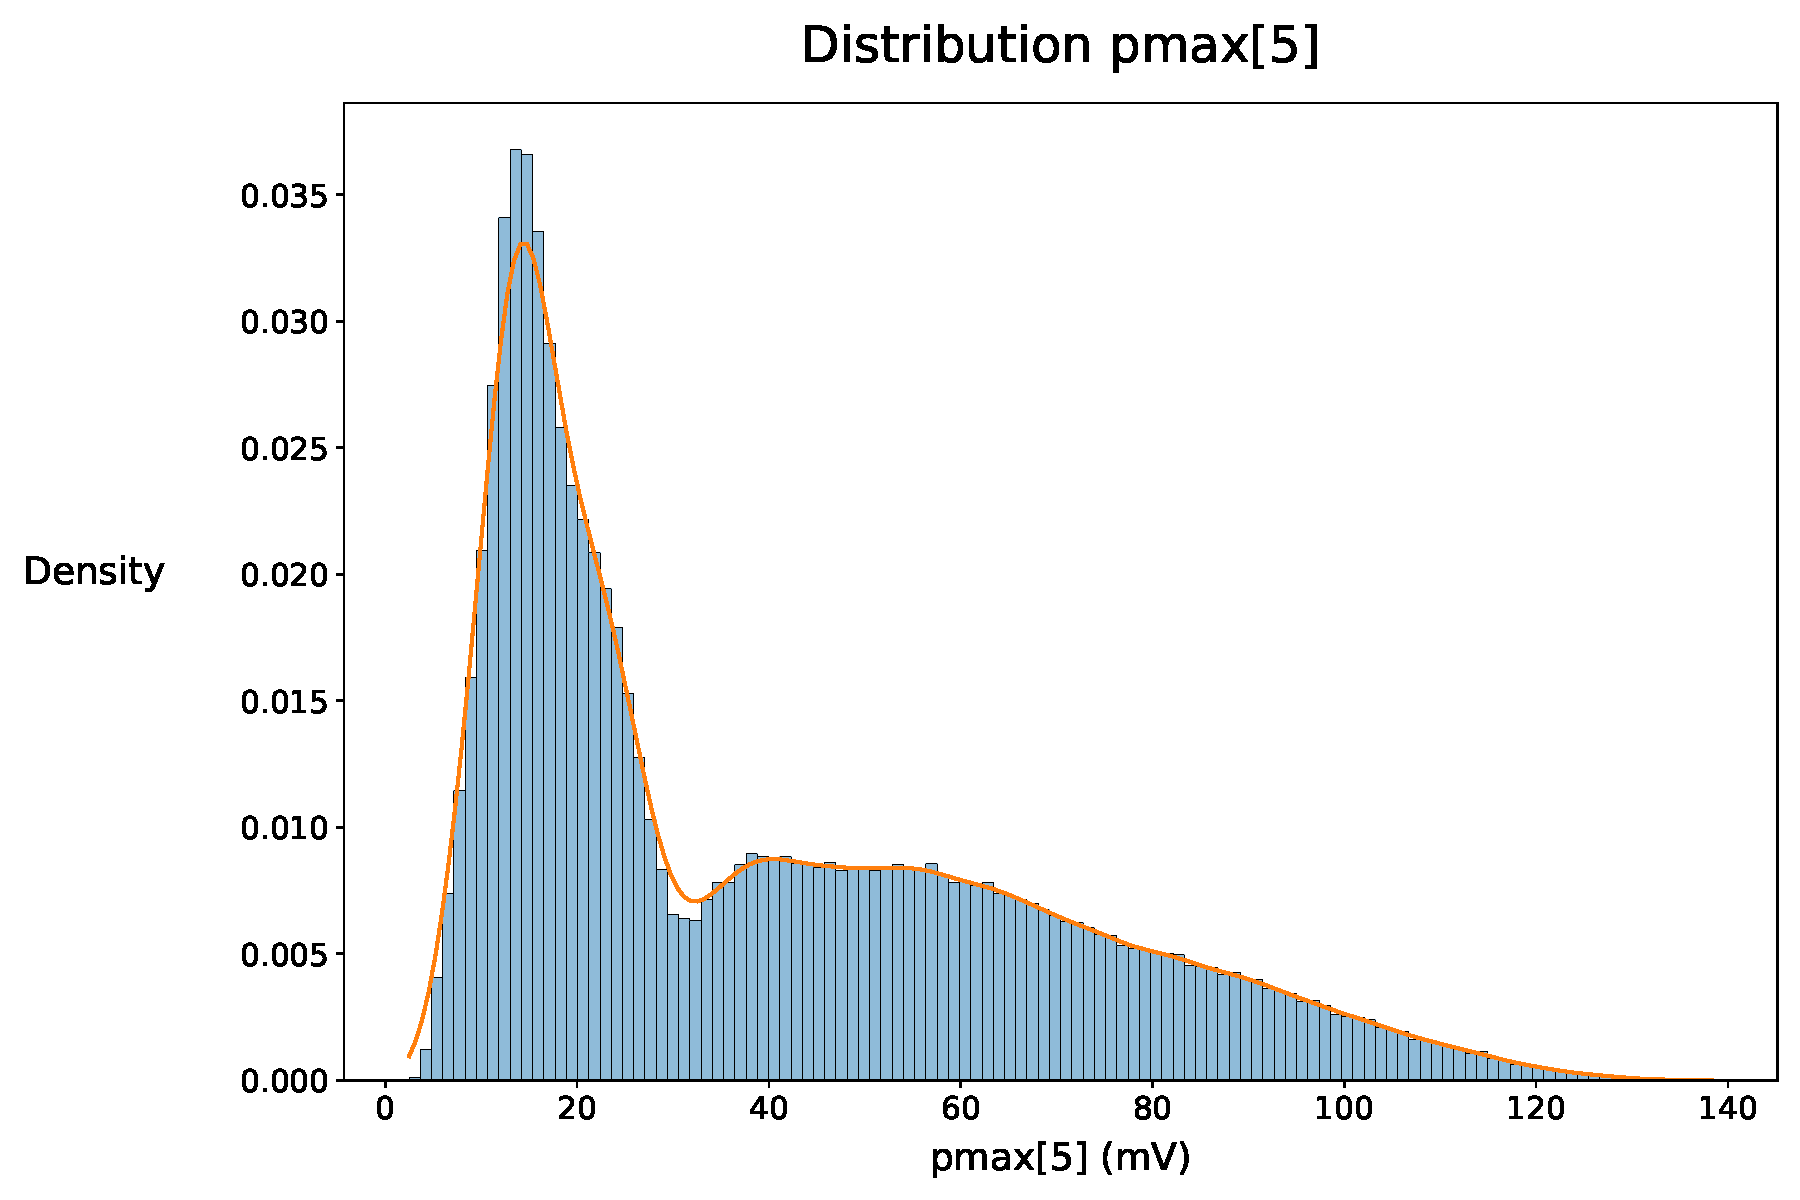
\includegraphics[scale=0.30]{images/pmax[5]_distr.pdf}}
\caption{Distribution of the pmax[5] values in the development set}
\label{fig:pmax[5]_distr}
\end{figure}
The difference between the noise and the signal can be also observed in the distributions of the values. A typical pmax probability function is represented in Figure \ref{fig:pmax[5]_distr}. The noise signals have completely different shapes and range of values. Most of the values have a low magnitude. This occurs because most of the time the pad is distant from the passing position.\\

The same analyses were performed on the other types presented in the listing \ref{lst:typeFeature}. Similar results were obtained for negpmax, area, and tmax. This confirmed that the features that share the same trailing "[n]" derive from the same signal. The tmax fields give less clear visualizations than the other three. On the other hand, the heat maps of the rms values do not present any visual pattern and they are in the order of a few $mV$. The reason is that only a small portion of the signal is characterized by the peaks. Most of the time, the signal has a small magnitude influenced by the noise.\\

%\begin{figure}[htbp]
%\centerline{\includegraphics[scale=0.35]%{images/negpmax_boxplot.pdf}}
%\caption{Negpmax boxplots}
%\label{fig:negpmax_boxplots}
%\end{figure}
Another consideration that can be made is on the distributions of negpmax. The density functions have an unusual number of outliers compared to the other features. 

\section{Proposed approach}
\subsection{Preprocessing}

\begin{figure}[htbp]
\centerline{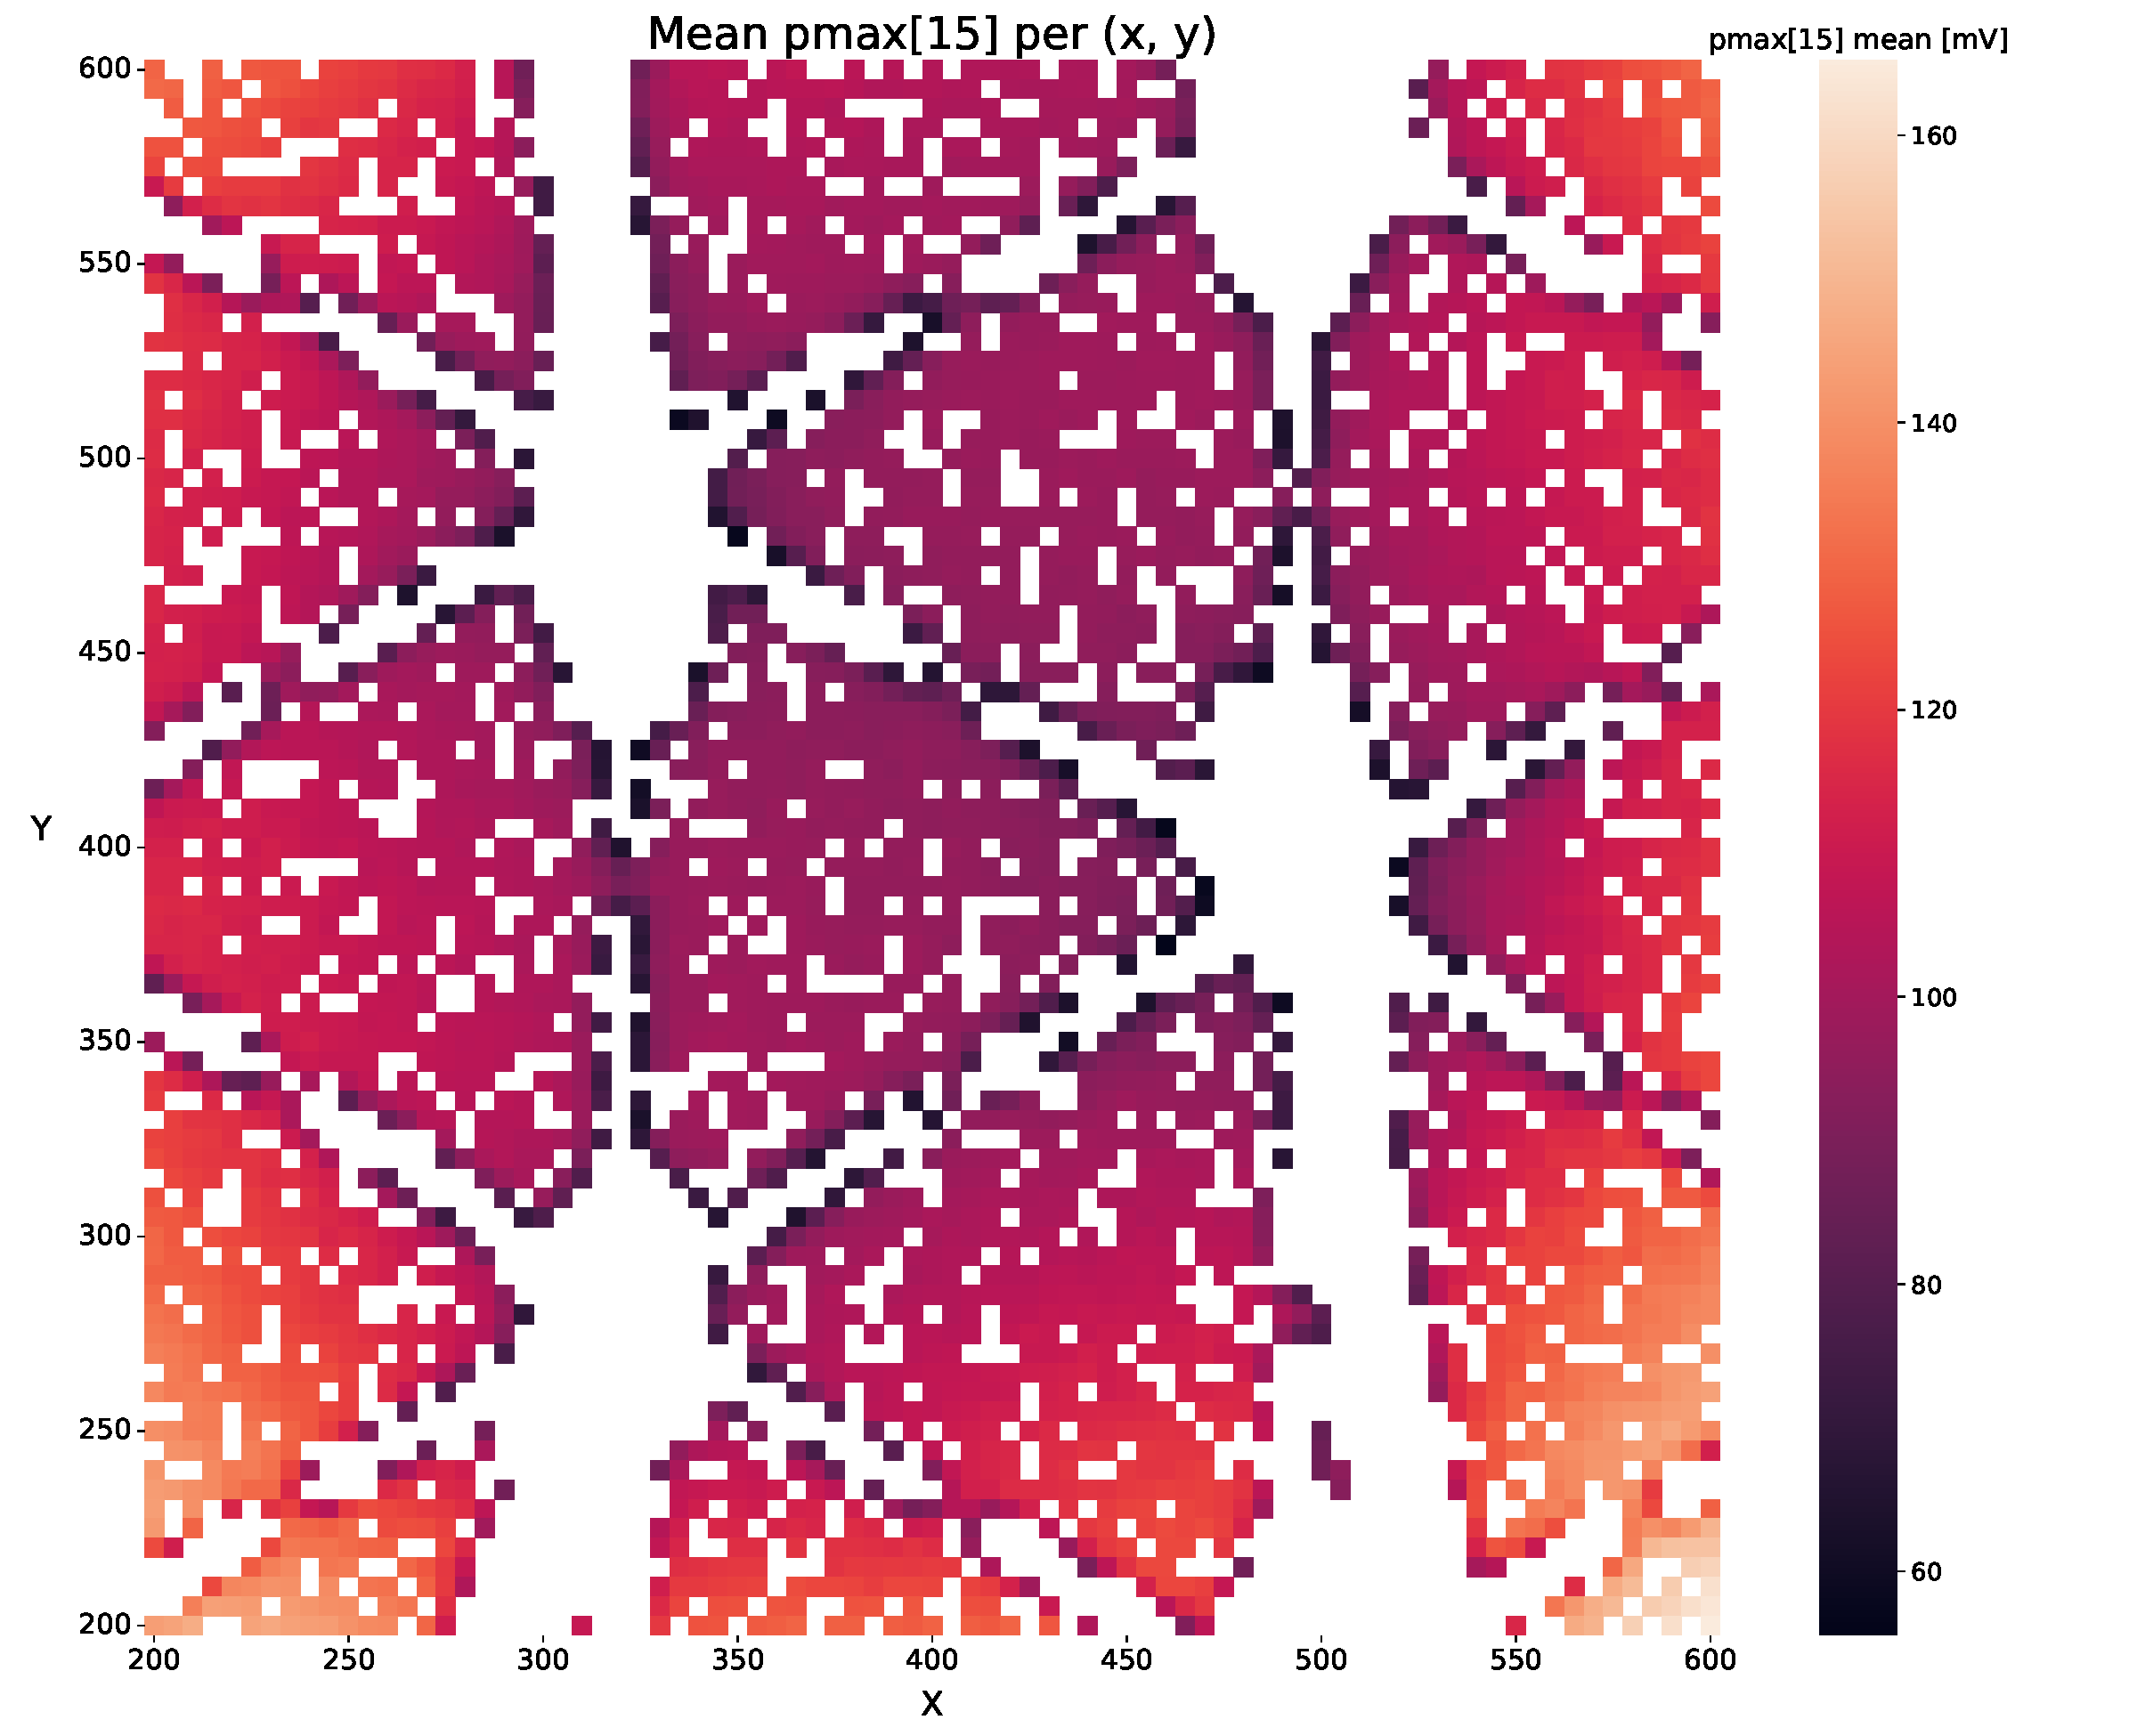
\includegraphics[scale=0.38]{images/pmax[15]_heatmap.pdf}}
\caption{Mean pmax[15] values aggregating by (x, y) the development set}
\label{fig:pmax[15]_heatmap}
\end{figure}
We have seen from a visual perspective, which are the features that contain most of the information. These intuitive considerations were confirmed by an analysis of the importances obtained by a Random Forest regressor with default parameters. Only the pmax, negpmax, and the area of the signal derived from the pads were significantly used by the algorithm.\\ 
An interesting exception is the signal 15. Even if it should be only random noise, the $pmax[15]$ is taken into consideration. Observing Figure \ref{fig:pmax[15]_heatmap}, we see that the values are on average higher on the borders of the sensor and lower near the pads. Therefore, it contains useful information that can be used by the models. \\
For these reasons, we kept only pmax, negpmax, and the area of the signal corresponding to a pad and the feature $pmax[15]$.\\


In Section \ref{sec:problemOverview}, we have observed that only the columns of type negpmax contain many outliers. The magnitude of them is very different from the rest of the values. The same is not valid for the rest of the features.
We have also discussed that the absolute values are higher when the passing position is close to the sensor. Due to the broad range of x and y, often this does not happen. \\ 
To avoid the removal of useful data, we used the following procedure: we detected and saved the minimum negpmax for each row, and then we analyzed them using the Tukey's Fences method for outlier detection with coefficient k equal to 3. \\
The first step takes the measurements of the nearest pad for each event. In this way, we detected and removed the rows that contained negpmax values extremely different even for the closest pad.
 
\subsection{Model selection}
We have tested the following models:
\begin{itemize}
    \item Random forest(RT): it is an ensemble machine learning technique used for classification and regression. During the training phase, several decision trees are created on different random datasets, sampled with replacement from the original data. For a regression problem, the output of the random forest is the mean of the predictions of the single decision trees. Every split is learned during training considering a criterion, e.g. mean squared error, and possibly on a random subset of the features \cite{randomForest} \cite{extraTree}.\\
The usage of multiple decision trees leads to a model more robust to noise \cite{randomForest}. The performance and the training times depend on the number of decision trees. The improvement provided by an increase in the number of decision trees is significant up to a certain number \cite{limitNumTrees}.\\
Even if the model is not as interpretable as a decision tree, the overall importance of the features can still be obtained.
\item Extra trees regressor(ET): it is an ensemble machine learning technique. There are only two main differences with the random forest method. The first is that every decision tree is built using the whole learning sample. The second is that every split is randomly selected from a uniform distribution inside the candidate feature's empirical range. Then among all the random splits, the best one is chosen and used to grow the tree. \\
The computational efficiency of the algorithm is an important advantage of this model \cite{extraTree}.
\item Voting regressor(VR): it is an ensemble machine learning technique. It is based on the simple idea of combining the output of different regression models. In this way, the advantages of multiple models can be incorporated. In this case, we used the mean of the random forest and the extra trees regressors. %TODO: cite a paper and change the name, I don't think that voting regressor is the official one
\end{itemize}
\subsection{Hyperparameters tuning}
The tuning was performed on the parameters of the RT and the ET. As a consequence, the voting regressor used the best performing configurations of the other two models. \\
The RT and the ET algorithms share all the parameters we considered for the tuning. The parameters and their values are in Table \ref{tab:tabHP}.
\begin{table}[h]
    \centering
    \caption{Hyperparameters considered}
    \label{tab:tabHP}
    \begin{tabular}{|c|c|c|}
        \hline
        \textbf{Model} & \textbf{Prameters} & \textbf{Values} \\
        \hline
        &$n\_estimators$&\{72, 100, 128\}\\
        Random Forest&$max\_depth$&\{None\footnote[1]{}, 30, 22\}\\
        &$max\_features$&\{sqrt, 1.0\}\\
        &$criterion$&squared\_error\\
        \hline
        &$n\_estimators$& \{72, 100, 128\} \\
        Extra trees&$max\_depth$&\{None\footnote[1]{}, 33, 25\}\\
        &$max\_features$&\{sqrt, 1.0\}\\
        &$criterion$&squared\_error\\
        \hline
    \end{tabular}
\end{table}

Over a certain threshold, increasing the number of trees does not improve significantly the performances, while extending considerably the computational time.  The range $[64, 128]$ is suggested in many datasets\cite{limitNumTrees}. Also for this problem, it is not worth using over 128 estimators. \\
For this reason, we tested values of n\_estimators near 100. \\

The maximum depth obtained by the RT and the ET with default parameters is respectively 38 and 41. We tested the configurations with the maximum depth: None\footnote[1]{It does not impose any limits to the maximum depth of the trees}, 60\%, and 80\% of the previous values. 

We divided the development dataset with a split 80/20. On the 80\%, we performed a cross validation using 4 folds. The metric used was the average Euclidean distance (\ref{eq:EuclideanDist}).\\
The 20\% was used to test the best performing models, before using all the labeled data to build the final regressors.
\section{Results}
\label{seq:results}
%The feature selection process brought an important improvement to our solution, after the removal of the features that we decided to discard during the features analysis,
%our solution went from 5.039 to valore.
%5.039 Soluzione online base
%Distance on local test combined : 4.677499770610218
%Distance on local test randomF : 4.6320736739355395
%Distance on local test ET : 5.03086466714152
%Adding then the maximum pmax and the normalized pmax for each event improves our solution locally and on the online score board, the results we obtain

The tuning showed that for RF and ET the best hyperparameter configurations are very similar, the only difference is max\_features, 1.0 for ET, and $sqrt$\footnote[1]{It considers only $\sqrt{num\_features}$ features while searching for the best split} for RF.
The best configurations are shown in Table \ref{tab:tabBestConf}.
\begin{table}[h]
    \centering
    \caption{Best hyperparameter configurations}
    \label{tab:tabBestConf}
    \begin{tabular}{|c|c|c|c|c|}
        \hline
        \textbf{Model} & \textbf{n\_estimators} & \textbf{criterion} & \textbf{max\_features} & \textbf{max\_depth} \\
        \hline
        RF & 128 & squared\_error & sqrt & None \\
        \hline
        ET & 128 & squared\_error & 1.0 & None \\
        \hline
    \end{tabular}
\end{table}

Each step of the pipeline improved the performances of the models. The final result on the public leaderboard is $4.614 \mu m$\footnote[2]{The training of the final models is done on all the labeled dataset}, while the score obtained by only training the regressors on the original development set, without preprocessing and hyperparameter tuning, is $5.039 \mu m$.\\
After the tuning, we observed locally\footnote[3]{Local results are computed on an 80/20 train/test split} an average distance of $4.141 \mu m$, $3.830 \mu m$, and $3.897 \mu m$, respectively for RT, ET, and VR. On the other hand, the best online score is obtained by VR. A possible explanation is that VR, exploiting the advantages of the other two regressors, performs better on points $(x, y)$ not present in the training set.\\

Our public result is in the first third of the public leaderboard. Better results are achievable, but they are possibly obtained with different models. Furthermore, our models give a score that is considerably better than the leaderboard baseline: the improvement in the distance is $2.015 \mu m$.\\
We also made a comparison with a naive regressor. This model just predicts the average between $x_{max}$ and $x_{min}$, where $x_{max}$ is the maximum value of $x$ in the development dataset and $x_{min}$ is the minimum. It proceeds in the same way for $y$.
This approach reaches a public score of $242.693 \mu m$. It is orders of magnitude worse than our solution. \\



\section{Discussion}
Among the three models, the VR achieves the best performance. This is what we expected since the VR exploits the advantages of the regressors it uses. Moreover, it can be noted that the points immediately near the pads are more difficult to predict(see Figure \ref{}).\\ 
% contains the mean distance\footnotemark[2] per $(x, y)$. .\\

Further tests could take into consideration a broader grid search, with more configurations and parameters. Also, the proposed approach does not take into account domain knowledge of particles and of the RSD sensor. They could be used to improve the pipeline. Additionally, other types of models, such as Neural Networks, could be examined.\\
Nevertheless, we are satisfied with our solution, which outperforms both a naive regressor and the leaderboard baseline.


\bibliography{bibliography}
\bibliographystyle{ieeetr}

\end{document}
